\chapter{Overview}
\label{chp:overview}

\GrG\ is combined from two groups of components:
The first consists of the compiler \texttt{grgen} and two runtime libraries, which offer the basic functionality of the system;
the compiler transforms specifications of declarative graph rewrite rules into highly efficient .NET-assemblies.
The second consists of the interactive command line \texttt{GrShell} and the graph viewer \texttt{yComp},
which offer a rapid prototyping environment supporting graphical and stepwise debugging of rules that are controlled by sequences.

%%%%%%%%%%%%%%%%%%%%%%%%%%%%%%%%%%%%%%%%%%%%%%%%%%%%%%%%%%%%%%%%%%%%%%%%%%%%%%%%%%%%%%%%%%%%%%%%
\section{System Overview}\indexmain{overview, system}\label{systemoverview}

Figure~\ref{figsys} gives an overview of the \GrG\ system components and the involved files.

\begin{figure}[htbp]
  \centering
  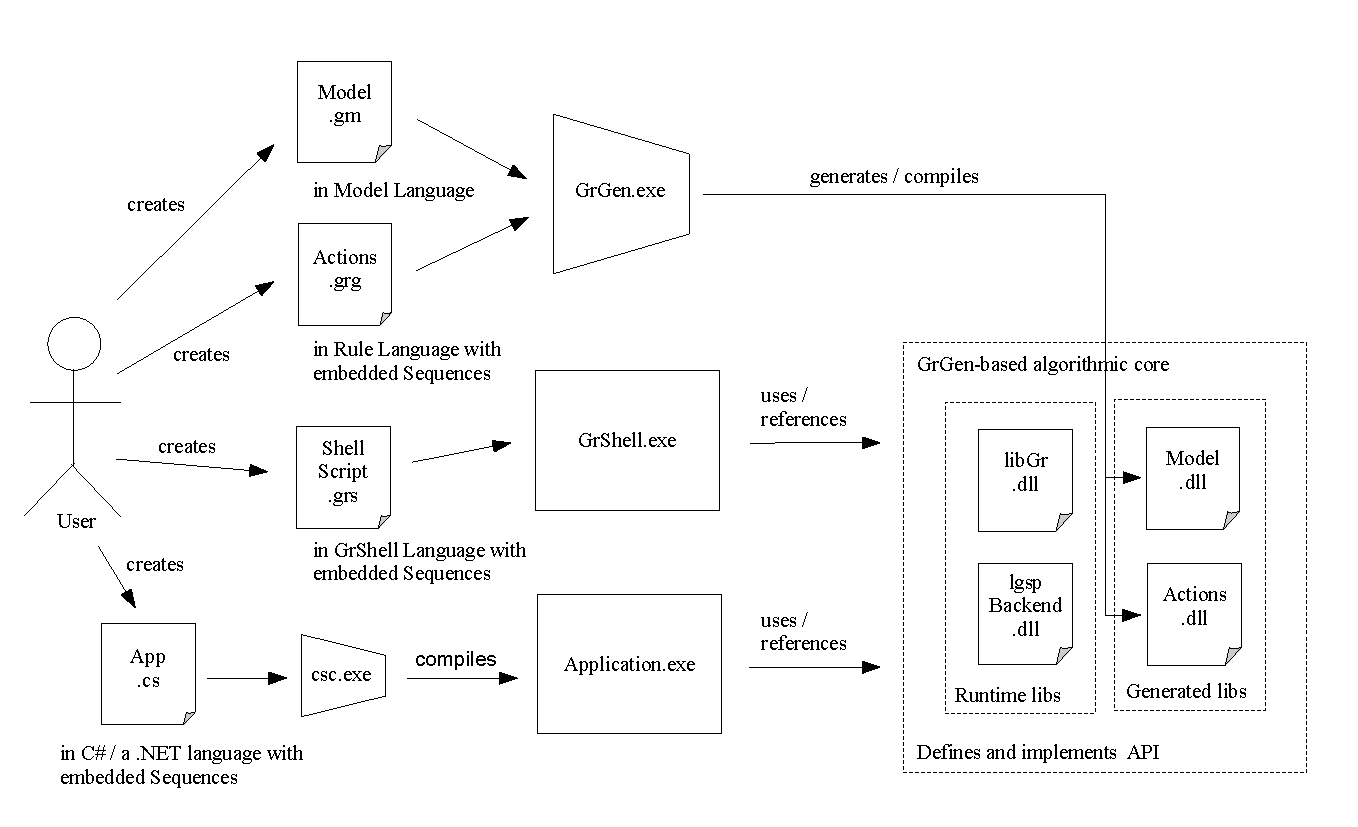
\includegraphics[width=\textwidth]{fig/OverviewGenerationArtefacts}
  \caption{\GrG\ system components and artifacts}
  \label{figsys}
\end{figure}

A graph rewrite system\footnote{In this context, system is less a grammar rewrite system, but rather a set of interacting software components.} is \emph{defined} by a rule set file (\texttt{*.grg}, written in the rule and computations language), which may include further rule set files, and use zero or more graph model description files (\texttt{*.gm}, written in the model language).
Executable code is \emph{generated} from these specifications by \texttt{GrGen.exe}; 
the generated parts are assisted by the \emph{runtime libraries} \texttt{libGr} and \texttt{lgspBackend}.
Together they form the system that can be used via an \emph{API} by arbitrary .NET-applications, for the processing of a graph-based representation.
One application employing the \indexed{API} is shipped with \GrG, the \emph{shell} application \GrShell.
It may be used interactively, esp. for debugging, or may be scripted (in the shell language, which allows via \texttt{libGr} to execute sequences, a concise language offered to control rule applications).

Figure~\ref{process} depicts the major runtime objects.

\begin{figure}[htbp]
  \centering
  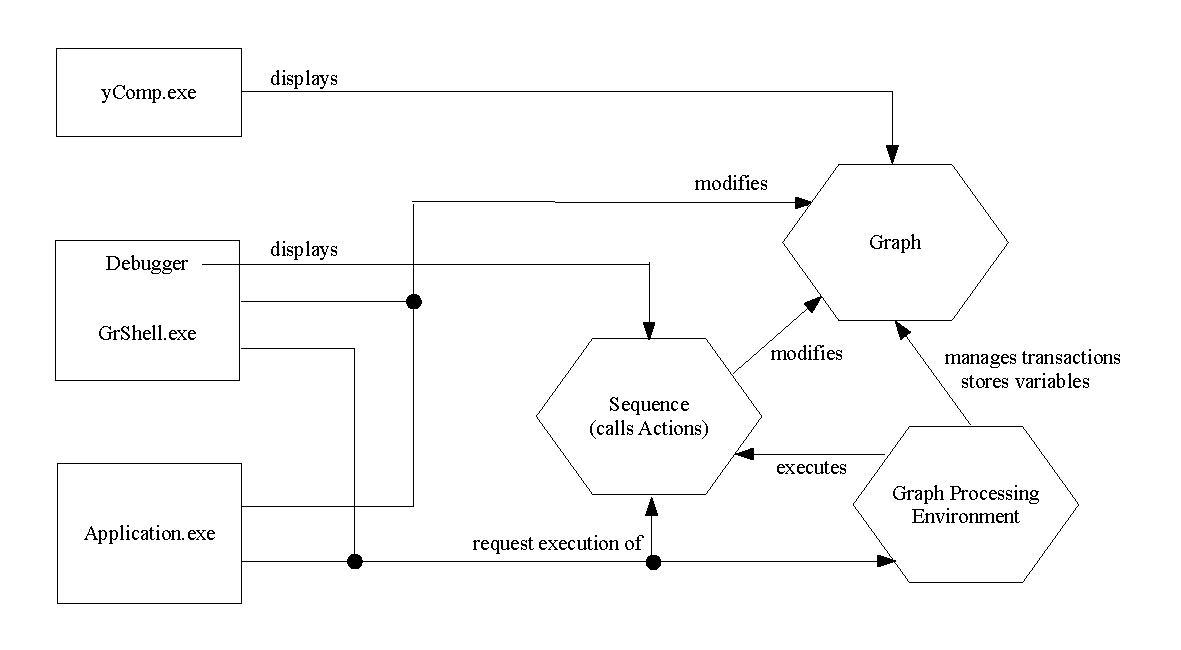
\includegraphics[width=\textwidth]{fig/OverviewRuntimeArtefacts}
  \caption{\GrG\ major runtime objects}
  \label{process}
\end{figure}

The central object is the \emph{graph}, it adheres to the specified graph model.
(In general you have to distinguish between a graph model on the meta level, a host graph created as instance of the graph model, and a statically specified pattern graph of a rule that matches a portion of the host graph at runtime).
It may be modified directly by \GrShell, or by a user application.
But typically is it changed by the application of one of the generated \emph{actions}, most often from within a \emph{sequence}, which is parsed into an operator tree and then interpreted, by the graph \emph{processing environment}.
The processing environment maintains the global variables in addition, and modifies the graph directly in case of transaction rollback (based on the graph change events recorded since transaction start).

The \GrShell\ is a readily available execution environment that is sufficient for mapping tasks that require only console or file output.
But even when you want to integrate a graph based algorithmic core into your existing .NET application, 
or are forced to write one because you must supply a long-running application reacting to events from the environment, esp. to user input,
may you be interested in additionally using the \GrShell\ because of its debugging abilities.
Employing the graph viewer \yComp\ it can visualize the graph at any time during execution.
Moreover, it can visualize the application of a rule, highlighting the matched pattern in the host graph, and the changes carried out.
It can do so for actions executed from a sequence, which can be executed step-by-step, under debugger control, highlighting the currently executed rule in the sequence.

%%%%%%%%%%%%%%%%%%%%%%%%%%%%%%%%%%%%%%%%%%%%%%%%%%%%%%%%%%%%%%%%%%%%%%%%%%%%%%%%%%%%%%%%%%%%%%%%
\section{The Tools}

All the programs and libraries of \GrG\ are open source licensed under \indexed{LGPL}.
Notice that the \yComp\ graph viewer is not a part of \GrG ; \yComp\ ships with its own license granted by \yFiles\ for academic use.
\yComp\ is closed-source and only free for non-commercial use --
this means above all that you are not allowed to ship it with a release of your own commercial software, in contrast to the \GrG\ libraries.

Executing a generated graph rewrite system requires .NET 2.0 or later; compiling and debugging a graph rewrite system in addition requires JAVA 1.5 or later. 
You find the tools in the \texttt{bin} subdirectory of your \GrG\ installation.
%\pagebreak

%-----------------------------------------------------------------------------------------------
\subsection{\texttt{\indexed{GrGen.exe}}} \label{grgenoptions}

\parpic[l] {

\includegraphics[width=48pt]{fig/grgen-256.png}
}
\noindent The \texttt{GrGen.exe} assembly implements the \GrG\ generator.
The \GrG\ generator parses a rule set and its model files and compiles them into .NET assemblies.
The compiled assemblies form a specific graph rewriting system together with the \GrG\ backend.

\begin{description}
  \item[Usage] \begin{tabular*}{\linewidth}{@{}l@{}l}\texttt{[mono] GrGen.exe } & \texttt{[-keep [<dest-dir>]] [-use <existing-dir>] [-debug]}\\
        &\texttt{[-b <backend-dll>] [-o <output-dir>] [-r <assembly-path>]}\\
        &\texttt{[-lazynic] [-noinline] [-profile]}\\
        &\texttt{[-statistics <statisticsfile>]}\\
        &\texttt{<rule-set>}\end{tabular*}
    \emph{rule-set} is a file containing a rule set specification according to Chapter~\ref{chaprulelang}. Usually such a file has the suffix \texttt{\indexed{.grg}}. The suffix \texttt{.grg} may be omitted.
By default \GrG\ tries to write the compiled assemblies into the same directory as the rule set file. This can be changed by the optional parameter \emph{output-dir}.
  \item[Options] \mbox{}
    \begin{tabularx}{\linewidth}{lX}
      \texttt{-keep} & Keep the generated C\# source files. If \emph{dest-dir} is omitted, a subdirectory \texttt{tmpgrgen$n$}\footnote{$n$ is an increasing number.} within the current directory will be created. The destination directory contains:
\begin{itemize}
  \item \texttt{printOutput.txt}---a snapshot of \texttt{stdout} during program execution.
  \item \emph{Name}\texttt{Model.cs}---the C\# source file(s) of the \emph{rule-set}\texttt{Modell.dll} assembly.
  \item \emph{Name}\texttt{Actions\_intermediate.cs}---a preliminary version of the C\# source file of the \emph{rule-set}'s actions assembly.
	This file is for internal debug purposes only (it contains the frontend actions output).
  \item \emph{Name}\texttt{Actions.cs}---the C\# source file of the \emph{rule-set}\texttt{Actions.dll} assembly.
\end{itemize}\\
      \texttt{-use} & Don't re-generate C\# source files. Instead use the files in \emph{existing-dir} to build the assemblies.\\
      \texttt{-debug} & Compile the assemblies with debug information.\\
      \texttt{-lazynic} & Negatives, Independents, and Conditions are only executed at the end of matching (normally asap).\\
      \texttt{-noinline} & Subpattern usages and independents are not inlined.\\
      \texttt{-profile} & Instruments the matcher code to count the search steps carried out.\\
      \texttt{-statistics} & Generate matchers that are optimized for graphs of the class described by the \emph{statisticsfile} (see \ref{custom} on how to save such statistics).\\
      \texttt{-b} & Use the backend library \emph{backend-dll} (default is LGSPBackend).\\
      \texttt{-r} & Link the assembly \emph{assembly-path} as reference to the compilation result.\\
      \texttt{-o} & Store generated assemblies in \emph{output-dir}.
    \end{tabularx}
  \item[Requires] .NET 2.0 (or above) or Mono 1.2.3 (or above). Java Runtime Environment 1.5 (or above).
\end{description}

\begin{note}
Regarding the column information in the error reports of the compiler please note that tabs count as one character.
\end{note}

\begin{note}
As .NET supports integration with native code, you may even use a \GrG-generated graph rewriting kernel from a native application.
\end{note}

\begin{note}\label{note:modelruledump}
The grgen compiler consists of a Java frontend used by the C\# backend \texttt{grgen.exe}.
The java frontend can be executed itself to get a visualization of the model and the rewrite rules,
in the form of a dump of the compiler IR as a .vcg file:\\
\texttt{java -jar grgen.jar -i yourfile.grg}
\end{note}

\begin{note}
If you run into \texttt{Unable to process specification: The system cannot find the file specified} errors, 
grgen is typically not able to execute the JAVA frontend.
Check whether your path contains a zombie java variable from an old installation pointing to nowhere; remove it in this case.
Installing a JDK to a non system path and adding the bin folder of the JDK to the path variable may help.
(Normally just installing a JRE is sufficient.)
\end{note}

%\pagebreak

%-----------------------------------------------------------------------------------------------
\subsection{\texttt{\indexed{GrShell.exe}}}

\parpic[l] {
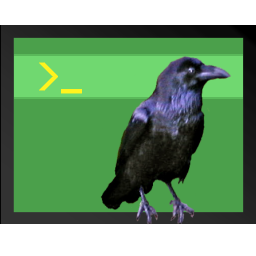
\includegraphics[width=48pt]{fig/grshell-256.png}
}
\noindent The \texttt{GrShell.exe}\indexmain{GrShell} is a shell application on top of the \LibGr.
\GrShell\ is capable of creating, manipulating, and dumping graphs as well as performing graph rewriting with graphical debug support.
For further information about the \GrShell\ language see Chapter~\ref{chapgrshell}.

\begin{description}
  \item[Usage] \texttt{[mono] grShell.exe [-N] [-SI] [-C "<commands>"] <grshell-script>*} \\
     Opens the interactive shell. The \GrShell\ will include and execute the commands in the optional list of \emph{grshell-script}s\indexmain{graph rewrite script} (usually \texttt{*\indexed{.grs}} files) in the given order.
	 The \texttt{grs} suffixes may be omitted. \GrShell\ returns 0 on successful execution, or in non-interactive mode -1 if the specified shell script could not be executed, or -2 if a \texttt{validate} with \texttt{exitonfailure} failed. This allows you to build a test-suite consisting of shell scripts.
  \item[Options] \mbox{}
    \begin{tabularx}{\linewidth}{lX}
      \texttt{-N} & Enables non-debug non-gui mode which exits on error with an error code instead of waiting for user input.\\
      \texttt{-SI} & Show Includes prints out to the console when includes are entered and left.\\
      \texttt{-C} & Execute the quoted \GrShell\ commands immediately (before the first script file). Instead of a line break use a double semicolon \texttt{;;} to separate commands. Take care that an exec inside such a command line needs to be exited with \indexed{\texttt{\#\S}} (to open and immediately close a shell comment, needed as exec terminator, because newline termination is not available here).
    \end{tabularx}
  \item[Requires] .NET 2.0 (or above) or Mono 1.2.3 (or above).
\end{description}

\begin{note}
The shell supports some \texttt{new set} configuration options that map to the \texttt{grgen} compiler flags (see \ref{sec:compilerconfigshell}), use them before any \texttt{new graph} commands so that matchers are generated according to the compiler flags you would use if you would execute the compiler directly.
\end{note}

\begin{example}
The \texttt{-C} option is often not as helpful as needed because bash splits the command given inside "" alongside spaces.
Unless you are a shell wizard in control of escaping and unescaping, you want to work with here documents.
The following example shell script from \texttt{examples/MovieDatabase-TTC2014} shows how to execute an \GrShell-script embedded as here document on all files in a folder.
\begin{grshell}
#!/bin/bash
for file in *.xmi; do	
    GrShell -N << HERE
import movies.ecore $file GrgenifyMovieDatabase.grg
redirect emit $file.grs
exec create_MovieDatabaseModel ;> [create_Movie] ;> [create_Actor] ;> [create_Actress] ;> [create_personToMovie]
redirect emit - 
validate exitonfailure exec noEdgesLeft
quit
HERE
done
\end{grshell}
\end{example}

%-----------------------------------------------------------------------------------------------
\subsection{\texttt{LibGr.dll}}
\label{sct:API}
The \LibGr\indexmain{libGr} is a .NET assembly implementing \GrG's \indexed{API}.
See the extracted HTML documentation for interface descriptions at \url{http://www.grgen.net/doc/API_4_4/};
a short introduction is given in chapter \ref{cha:api}.

%-----------------------------------------------------------------------------------------------
\subsection{\texttt{lgspBackend.dll}}
The \LGSPBackend\indexmain{lgspBackend} is a .NET assembly containing the libGr SearchPlan backend, the only backend supported by \GrG~as of now, implementing together with the generated assemblies the API offered by \LibGr.
It allows to analyze the graph and to regenerate the matcher programs at runtime, on user request, see \ref{custom}.
For a more detailed introduction have a look at chapter \ref{cha:developing}.

%-----------------------------------------------------------------------------------------------
\subsection{\texttt{yComp.jar}}
\label{tools:ycomp}
\yComp\indexmain{yComp} \cite{ycomp} is a graph visualization tool based on \yFiles\ \cite{yfiles}.
It is well integrated and shipped with \GrG, but it's not a part of \GrG.
\yComp\ implements several graph layout algorithms and has file format support for \indexed{VCG}, GML and YGF among others.
\begin{center}
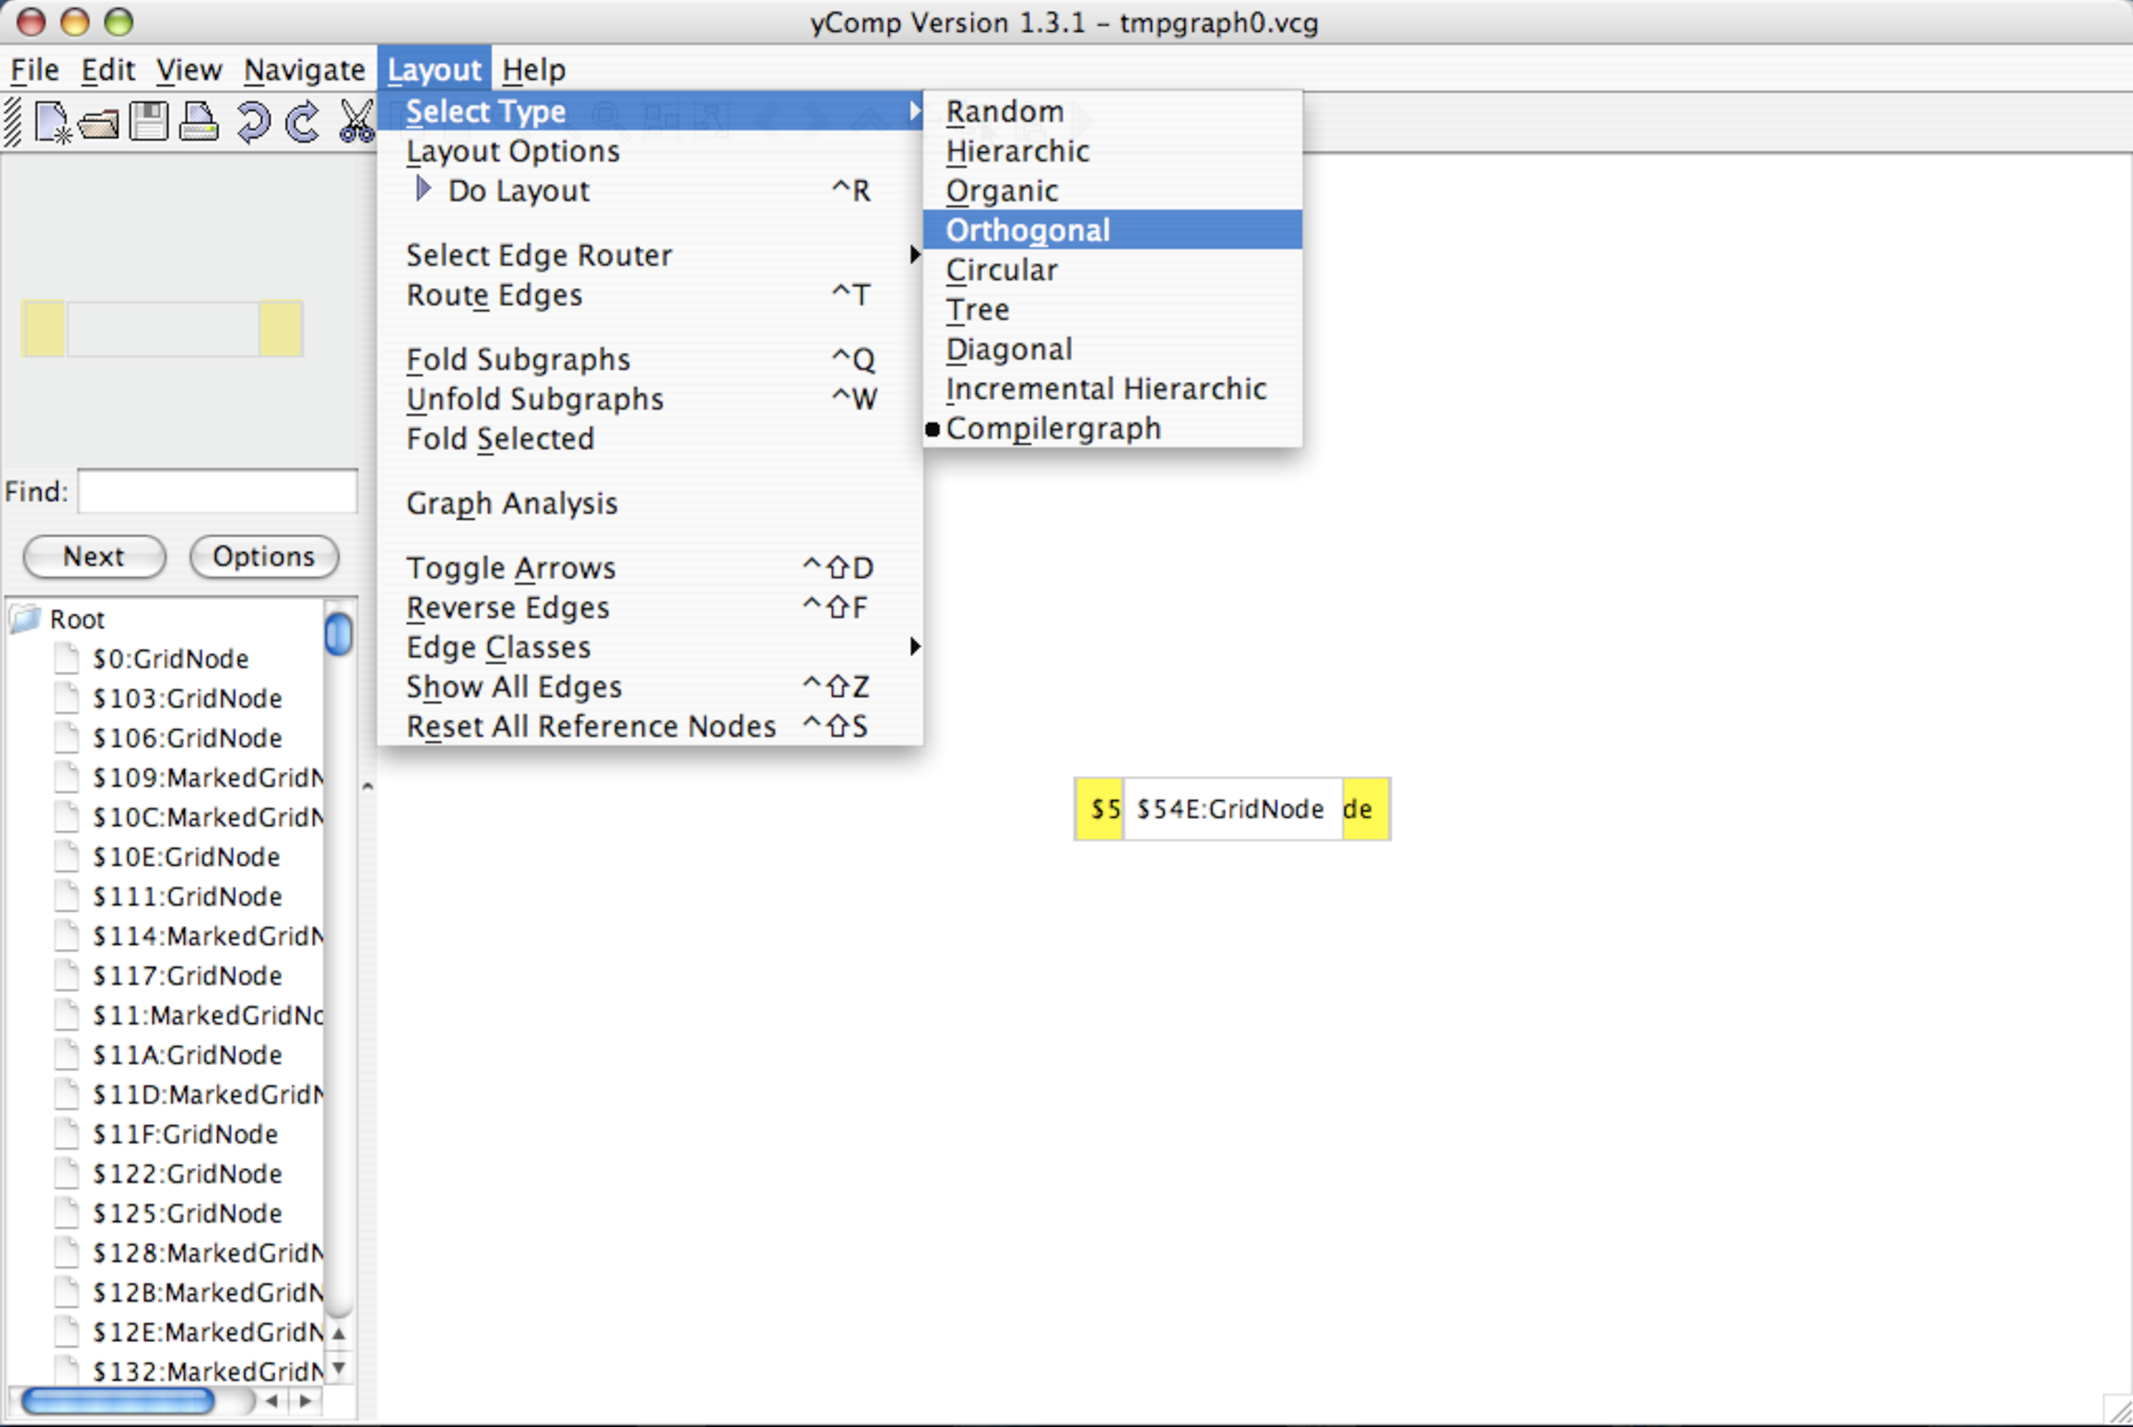
\includegraphics[width=0.49\linewidth]{fig/ycomp1.pdf} 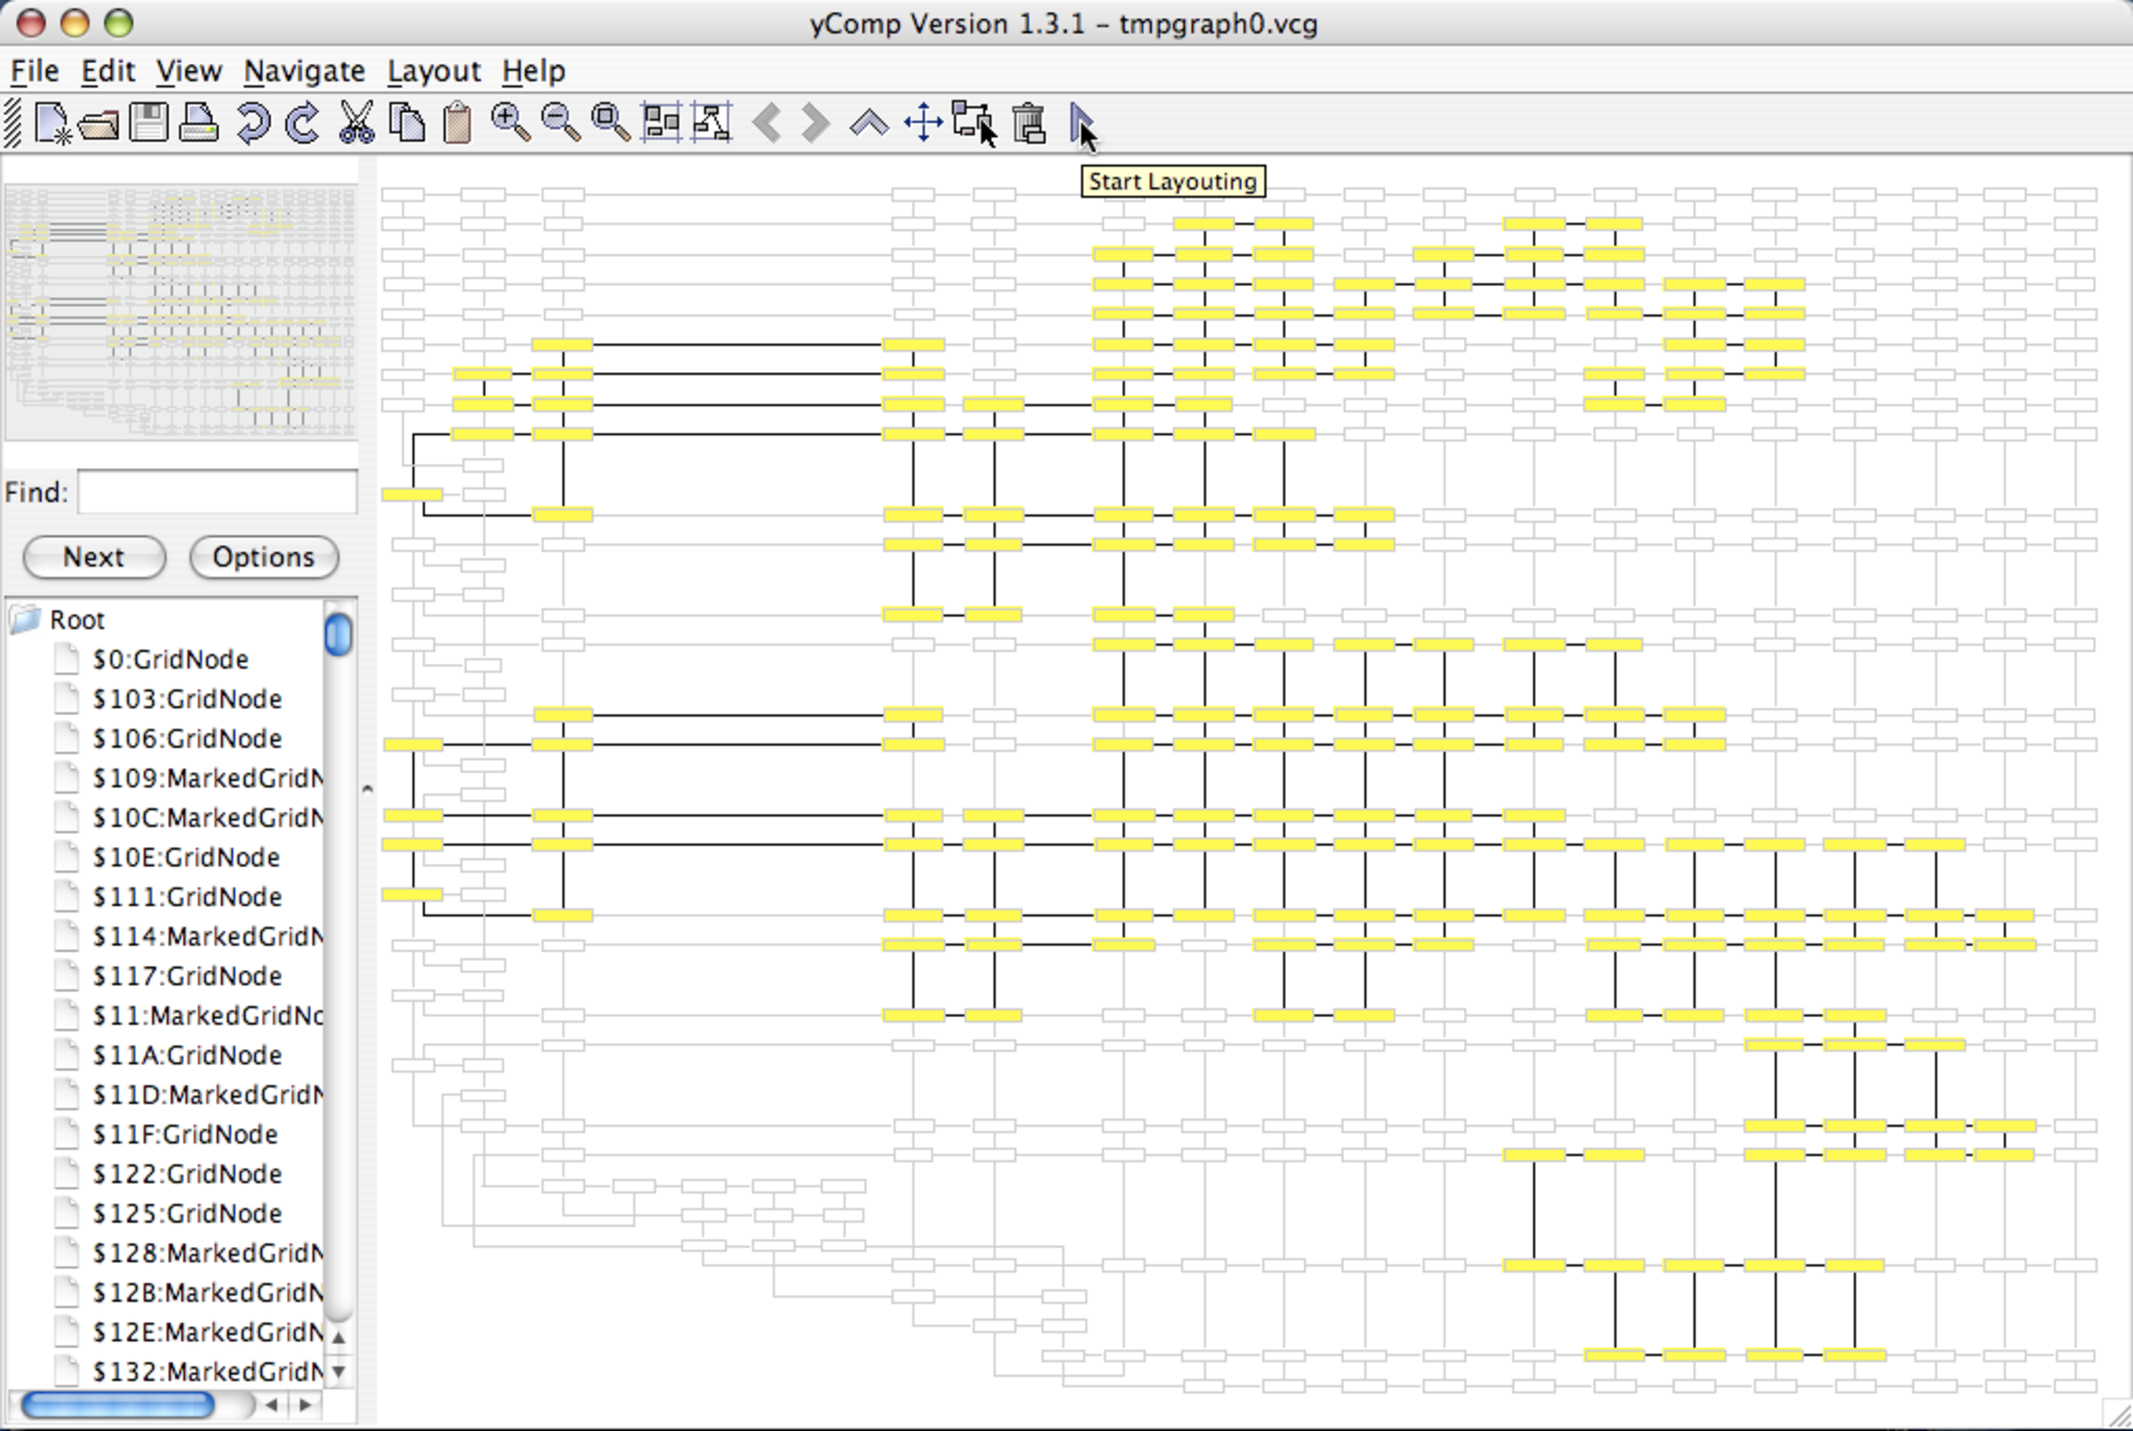
\includegraphics[width=0.49\linewidth]{fig/ycomp2.pdf}
\end{center}
\begin{description}
  \item[Usage] Usually \yComp\ will be loaded by the \GrShell. You might want to open \yComp\ manually by typing\\
   \texttt{java -jar yComp.jar [<graph-file>]}\\
  Or by executing the batch file \texttt{ycomp} under Linux / \texttt{ycomp.bat} under Windows,
  which will start \yComp\ on the given file with increased heap space.
  The \emph{graph-file} may be any graph file in a supported format. \yComp\ will open this file on startup.
  \item[Hints] The \indexed{layout algorithm}\indexmainsee{layout}{layout algorithm} \indexedsee{compiler graph}{layout algorithm} (\yComp's default setting, a version of \texttt{\indexedsee{hierarchic}{layout algorithm}} optimized for graph based compiler intermediate representations) may not be a good choice for your graph at hand.
  Instead \texttt{\indexedsee{organic}{layout algorithm}} or \texttt{\indexedsee{orthogonal}{layout algorithm}} might be worth trying.
  Use the rightmost blue play button to start the layout process. Depending on the graph size this may take a while.
  \item[Requires] Java Runtime Environment 1.5 (or above).
\end{description}


%%%%%%%%%%%%%%%%%%%%%%%%%%%%%%%%%%%%%%%%%%%%%%%%%%%%%%%%%%%%%%%%%%%%%%%%%%%%%%%%%%%%%%%%%%%%%%%%
\section{The Languages and their Features}\indexmain{features}

The process of graph rewriting at runtime can be divided into four steps:
Creating an instance graph according to a model,
searching a pattern aka finding a match,
performing changes to the matched spot in the host graph,
and, finally, selecting which rule(s) to apply where next.

This process is programmed at specification time utilizing a graph model language, a rule and computations language, and the sequences language for controlling rule applications.

%------------------------------------------------------------------------------------
\subsection{Graph Model Language}
At the foundation you find the graph model (meta-model) language given with \texttt{class} definitions in the style of an object-oriented language, with some influences of data definition languages as offered by databases. 

It allows you to specify \emph{node} and \emph{edge types}, with \emph{multiple inheritance} on the types (see Chapter \ref{chapmodellang}).
They are used in building a typed, directed multigraph (supporting multiple edges of the same type between two nodes).
In addition, you may declare undirected and arbitrarily directed edges; or may even register external types with \GrG.
Furthermore, connection assertions allow you to restrict the ``shape'' of the graphs.

Node and edge types can be equipped with \emph{typed attributes}, of the commonly known elementary types (integer and floating-point numbers, strings, booleans, and enums) or of some container types (available are hashmap and array based types).
In addition, methods supporting dynamic dispatch may be given.%(they are seldom needed for tasks based on graph-representations, though). 

Moreover, you may configure indices (see Chapter \ref{sec:performance}): attribute indices for a quick lookup of a graph element based on the attribute value, or incidence count indices for a quick lookup based on the number of incident edges.
Several indices are already built-in and automatically used by the pattern matchers, notably the type index for quick lookups based on element type, and the incident elements index giving access to the neighbouring elements in constant time.

%------------------------------------------------------------------------------------
\subsection{Rule and Computations Language}
On top of the graph model language and at the heart of \GrG\ do you find the rule and computations language.

It supports pattern-based \emph{rules}, which are built by a \emph{pattern to be matched} and a \emph{rewrite} to be carried out; or put differently: a left-hand-side precondition pattern and a right-hand-side postcondition pattern (see Chapter \ref{chaprulelang}).
A pattern is described by \emph{graphlets}, a specification of nodes connected by edges in an intuitive, easily writable, easily readable, and \emph{easily changeable} syntax.
Complex patterns are combined from elementary patterns with \emph{nested patterns} (defining alternative, optional, multiple and iterated structures, or negative and independent application conditions, see Chapter \ref{cha:nested}) and \emph{subpattern} definitions and usages (see Chapter \ref{cha:sub}).
Besides those parts for \emph{declarative} processing of structural information are \emph{attribute conditions} (see Chapter \ref{cha:typeexpr}) and \emph{attribute evaluations} available, the former are expressions computing an output value by reading attributes of matched elements, the latter are statements changing attribute values with assignments. 

The attribute processing expressions and statements are in fact parts of a full-fledged \emph{imperative programming language} integrated with the declarative pattern-based rule language (see Chapter \ref{cha:computations}).
The \emph{expressions} can query the graph with a multitude of available functions in addition to reading the attributes of matched elements and carrying out computations with the attributes; they compute a value and can be abstracted into \emph{functions}.
The \emph{statements} support direct graph changes and supply control flow statements and def variable declarations in addition to the attribute assignments; they change the state and can be abstracted into \emph{procedures}.
You especially find subgraph operations for the processing of nested graphs, with subgraph extraction, subgraph comparison, and subgraph insertion (see Chapter \ref{cha:graph}). 

Pattern matching can be adjusted fine-grained with homomorphic matching for selected elements (with \texttt{hom} declarations, so they can match the same graph elements), overriding the default isomorphic matching, and with type constraints (forbidding certain static types or requiring equivalence of dynamic \texttt{typeof}s).

The rewrite part of a rule keeps, adds and deletes graph elements according to the SPO approach, as specified by element declarations and references in the LHS and RHS patterns (there are three additional rule application semantics available: DPO or exact patterns only or induced subgraphs only).
The rewrite part supports two modes of specification: A rule can either express the changes to the match (\texttt{modify}-mode, requiring deletion to be specified explicitly) or specify a whole new subgraph (\texttt{replace}-mode).

A rich bouquet of single element rewrite operations is available on top of the basic ones with \emph{retyping} aka relabeling, that allows to change the type of a graph element while keeping its incident elements, with the creation of new nodes/edges of only dynamically known types or as exact copies of other nodes/edges, and with node merging and edge redirection constructs (see Chapter \ref{chapadvanced}).
Besides changing the graph can you \texttt{emit} user-defined text to \texttt{stdout} or files (supporting model-to-text transformations; see Chapter \ref{cha:imperativeandstate}).

A special class of computations are available with the post-match filter functions (see Chapter \ref{sub:filters}), that allow to inspect and manipulate the set of matches found when applying a rule (with all bracketing). 
This way you can \emph{accumulate} information over the matches, or \emph{filter} the matches set for the most interesting matches.
Several filters for sorting and clipping are already supplied or can be generated automatically on request.
Symmetry reduction is available with a filter for duplicate matches due to permuted elements from automorphic patterns.

\GrG\ rules are \emph{modular} or \emph{local}: you just note down the functionality.
Typically it is smeared into graph traversal code of global visiting passes.
This limits the changes needed during development and maintenance, and together with the concise and easily editable patterns saves you from many large-scale tedious modifications that are normally needed in those cases.
You are still free to build local (or even global) passes by combining rules and tests (tests are rules with only a LHS pattern) utilizing \emph{parameters}: input and output parameters are supported by rules and tests, the subpatterns, and functions and procedures.
They are typically used to define and advance the location of processing in the graph, but they are also used for attribute computations.
In addition visited flags can be queried and written, for marking already processed elements.

Subpatterns allow for pattern reuse, and allow via subpattern \emph{recursion} to match substructures extending into \emph{depth} (e.g. iterated paths -- but for just checking an iterated path condition, i.e. the transitive closure of a relation, there are predefined and even more efficient functions available that can be simply called.)
Iterated patterns allow to match substructures splitting into \emph{breadth} (e.g multinodes).
Both combined allow to match \emph{entire tree like structures} within a single rule application. 
Subpatterns and nested patterns are matched from the outermost to the innermost patterns with \emph{recursive descent}, handing already matched elements down; on \emph{ascend}, they can \texttt{yield} elements found out to the \texttt{def} elements of their containing pattern.
The nested patterns and subpatterns also support \emph{nested rewrite parts}, so that complex structures are not only matched (parsing), but can also get rewritten (transduction) --- yielding \emph{structure directed transformation}, alongside structures defined by graphlets combined in an EBNF-grammar-like way\cite{EBNFAGTIVE}.

Those features and their optimized implementation (offering e.g. pattern matcher parallelization with a simple annotation) crown \GrG\ the king of graph pattern matching and rewriting, and allow you to process graph representations at their natural level of abstraction, with a flexibility and performance coming near to what you can achieve by programming things by hand.

A graph rewrite system described in those languages can be employed via an \emph{API} by .NET-applications, typically written in C\# (see Chapter \ref{cha:api}).
%The API is provided in two versions --- for one named and typed entities which get generated, and for the other a string and object based interface on top of it offered by \LibGr. The \LibGr-based API is needed to work with arbitrary systems.
The other way round you can include C\#-code into your specifications by using external types or calling external functions and procedures, as well as sequences (see Chapter \ref{chapextensions}).

%------------------------------------------------------------------------------------
\subsection{Rule Application Control Language}
On top of the rules and computations language do you find the \emph{sequences} language, for controlling the application of the rules (and procedures or functions), determining \emph{which rule} to apply \emph{where} next. 

This strategy language allows to determine the rule that is called next by its control operators and constructs (see Chapter \ref{cha:xgrs}).
The basic ones available are the \emph{sequential} and \emph{logical operators}, the \emph{decisions}, and the \emph{loops} (defining the control-flow orchestration).
The location where to apply a rule may be defined with \emph{parameters} handed into the called rules, and received back from them. 
The sequences support \emph{variables} to store the locations (for data-flow orchestration).
A rule may be applied for the \emph{first match} found, or for \emph{all matches} that are available with all-bracketing.

The sequences offer a \emph{computations} sublanguage that supports calling procedures and functions, basic graph querying and modification, visited flags management, and storages manipulation (see Chapter \ref{seqcomp}).
The first ones allow to bypass the rules of the layer below for simple tasks, and especially allow to extract, insert and compare subgraphs. 
Visited flags used in marking processed elements must be allocated and freed, the sequence computations are the right place to do so.
Most usages are related to \emph{storages} which are variables of container type storing graph elements, they esp. allow to build transformations following a wavefront running over the graph (see Chapter \ref{cha:container} for more on containers).

The sequences can be abstracted into a \emph{sequence definition} that can then be called in the place of a rule.
This way common parts can be reused, but especially is it possible to program a recursive strategy.
For simulation runs, several indeterministic choice operators are available.

Advanced constructs are available with \emph{transactions} angles and \emph{backtracking} double angles capable of \emph{rolling back changes} carried out on the graph to get back to the state of the graph again from before their nested content was applied (see Chapter \ref{cha:transaction}).
With them you can easily try things out without having to invest into programming the bookkeeping needed to revert to an old state.
They allow to systematically run through a search space, or even to enumerate a state space, materializing interesting states reached in time out into space.

Those sequences are available in an integrated form in the rule language (see Chapter \ref{cha:imperativeandstate}).
After applying the direct effects of a rule it is possible to apply an \emph{embedded sequence} for follow-up tasks that just can't be expressed with a single rule application; those sequences have access to the elements of their containing rule, they allow to build complex transformations with rule-sequence-rule call chains.
		
%------------------------------------------------------------------------------------
\subsection{Shell Language}
Those were the features of the languages at the core of the \GrG-System (implemented by the generator \texttt{grgen.exe} and the runtime libraries \texttt{libGr} and \texttt{lgspBackend}).
In addition, the \GrG\ system supplies a shell application, the \GrShell,
which offers besides some common commands, variable handling constructs, and file system commands several constructs for \emph{graph handling} and \emph{visualization}, as well as constructs for \emph{sequence execution} and \emph{debugging}.
Furthermore, some switches are available to configure the shell and the graph processing environment, as well as the \texttt{grgen} compiler.

Regarding graph handling you find commands for graph creation and manipulation, graph export and import, and graph change recording plus replaying (see Chapter \ref{chapgrshell}).
For graph creation 3 simple \texttt{new} commands are available, one for creating an empty graph, one for creating a node, and one for creating an edge (in between two nodes).
The GRS exporter serializes with the same syntax, which is also expected by the GRS importer.
Write a file in this simple format if the available import formats are not supported by your data source.

For direct graph manipulation you find deletion and retyping commands in addition to the creation commands, and commands for assigning attributes of graph elements.
Moreover, \texttt{export} and \texttt{import} commands are available for serializing a graph to a file, and for unserializing a graph from a file (in \texttt{GRS}, \texttt{GXL} and \texttt{XMI/ecore} formats). 
Changes that are occurring to a graph may be \texttt{record}ed to a \texttt{GRS} and later \texttt{replay}ed or simply \texttt{import}ed.
Change recording allows for post-problem debugging, but allows also to use \GrG\ as a kind of embedded database that persists changes as they appear. %(at the price of replaying changes that are rendered futile by later changes).

The graph and the model can be queried furtheron for e.g. the defined types (utilizing a reflection-like interface) or the attributes of a graph element.
The graph may be validated against the connection assertions specified in the model, or against a sequence that gets executed on a clone of the host graph.

Regarding sequence execution you find the central \texttt{exec} command that is \emph{interpreting} the following sequence (in fact by delegating the parsing and execution to \texttt{libGr}).
In addition, action \texttt{profile}s may be \texttt{show}n. They are available when \emph{profiling} instrumentation was switched on, telling about the number of search steps or graph accesses carried out.

The actions can be replaced at runtime by loading another actions library; the backend could be, but currently there is only one available, the \texttt{lgspBackend}.
This backend supports further custom commands, that start with a \texttt{custom graph} or \texttt{custom actions} prefix. 
They allow to \texttt{analyze} the graph in order to compile some statistics about the characteristics of the graph that are of relevance for the pattern matcher.
And in the following to re-generate the pattern matchers at runtime (\texttt{gen\_searchplans}) given the knowledge about the characteristics of the graph, yielding matchers which are \emph{adapted to the host graph} and thus typically faster than the default pattern matchers generated statically into the blue.
You can inspect the search plans in use with the \texttt{explain} custom command.

The debugger component of the \GrShell\ allows to \texttt{debug} a sequence \texttt{exec}ution step-by-step, highlighting the currently executed rule in the sequence, and displaying the current graph in the graph viewer \yComp;
in detail mode even the match found and the rewrite carried out by the rule are highlighted in the graph (see Chapter \ref{chapdebugger}).

The graph visualization is highly \emph{customizable}.
You can choose one from several available layout algorithms.
You can define e.g. the colors, the shapes of nodes, or the linestyle of edges, based on the type of the graph elements,
or exclude uninteresting types altogether from the display.
You can pick the attributes that are to be shown directly (normally they are only displayed on mouse-over).
Furthermore, you can configure \emph{visual graph nesting} by declaring edges as containment edges, thus keeping large graphs with containment or tree relations \emph{understandable}.
For large graphs that are beyond the capabilities of the graph viewer you can define that only the matches plus their context up to a certain depth are displayed.
Altogether, you can tailor the graph display to what you need, transforming an unreadable haystack which is what large graphs tend to become (if not rendered utilizing the means from above) into a well-readable representation.

